\documentclass[11pt]{beamer}
\usetheme{CambridgeUS}
\usepackage[utf8]{inputenc}
\usepackage[T1]{fontenc}
\usepackage[english]{babel}
\usepackage{amsmath}
\usepackage{amssymb, amsfonts, latexsym, cancel}
\usepackage{float}
\usepackage{graphicx}
\usepackage{epstopdf}
\usepackage{subfigure}
\usepackage{multicol}
\setbeamercovered{transparent}

\title[UI]{\bf\Huge User Interface}
\subtitle{Fundamentals to programming I}
\author[jrodriguezoc]{Joaquín Rodríguez Ocharán}
\institute[]{System Engineering School\\
System Engineering and Informatic Department\\
Production and Services Faculty\\
San Agustin National University of Arequipa}
\date{2020}
\logo{
\includegraphics[width=1.3cm]{images/unsaLetter}}
\titlegraphic{
\includegraphics[width=1.37cm]{images/unsaLogo}}

\begin{document}
	\begin{frame}
		\titlepage
	\end{frame}		
	
	\begin{frame}{Content}
		\tableofcontents
	\end{frame}
	
	\section{Introduction}
	\begin{frame}{Introduction}
		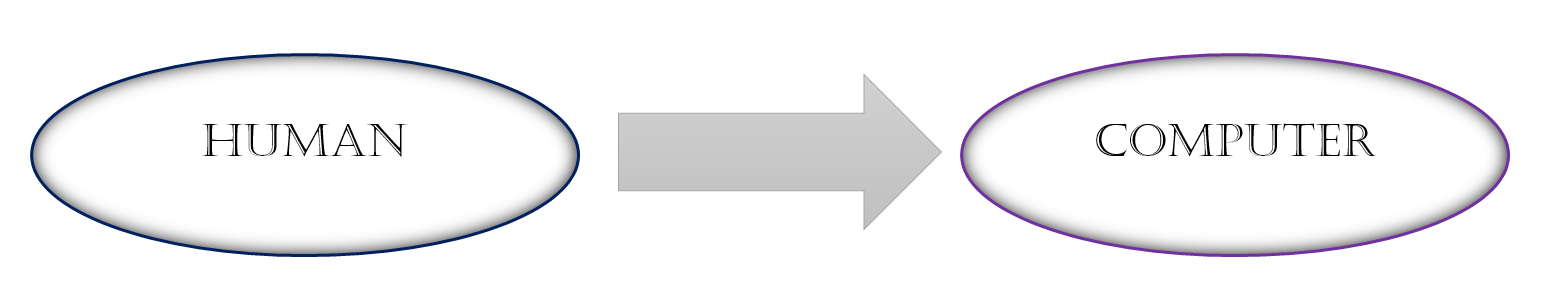
\includegraphics[width=11.7cm]{images/inter}
		The various types of user interfaces
		\begin{itemize}
			\item Graphical User Interface (GUI)
			\item Command Line Interface (CLI)
			\item Natural User Interface (NUI)
			\item Text User Interface (TUI)
			\item Voice User Interface (VUI)
		\end{itemize}
	\end{frame}
	
	\section{Graphic User Interface}
	\begin{frame}{Graphical User Interface (GUI)}
		\begin{center}
			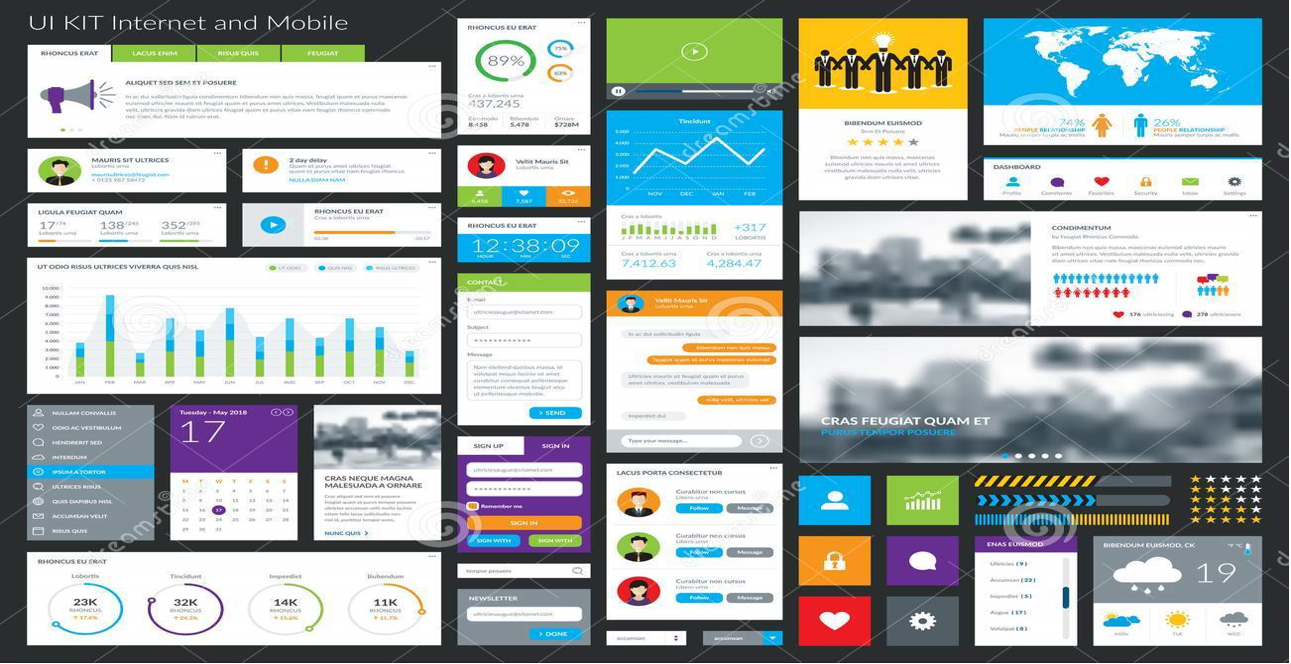
\includegraphics[width=10.5cm]{images/interMult2}
		\end{center}
	\end{frame}

	\section{Java}
	\begin{frame}{Java}
		\begin{block}{AWT(Abstract Window Toolkit)}
			\begin{itemize}
			\item Java 1.0
			\item Everything to the O.S
			\item Simple Graphics
			\end{itemize}
		\end{block}
		\begin{block}{SWING}
			\begin{itemize}
			\item Java 1.2
			\item All over a window
			\item Complicated Graphics
			\end{itemize}
		\end{block}
	\end{frame}
	
	\section{Hierarchy}
	\begin{frame}{Hierarchy of Swing JComponent}
		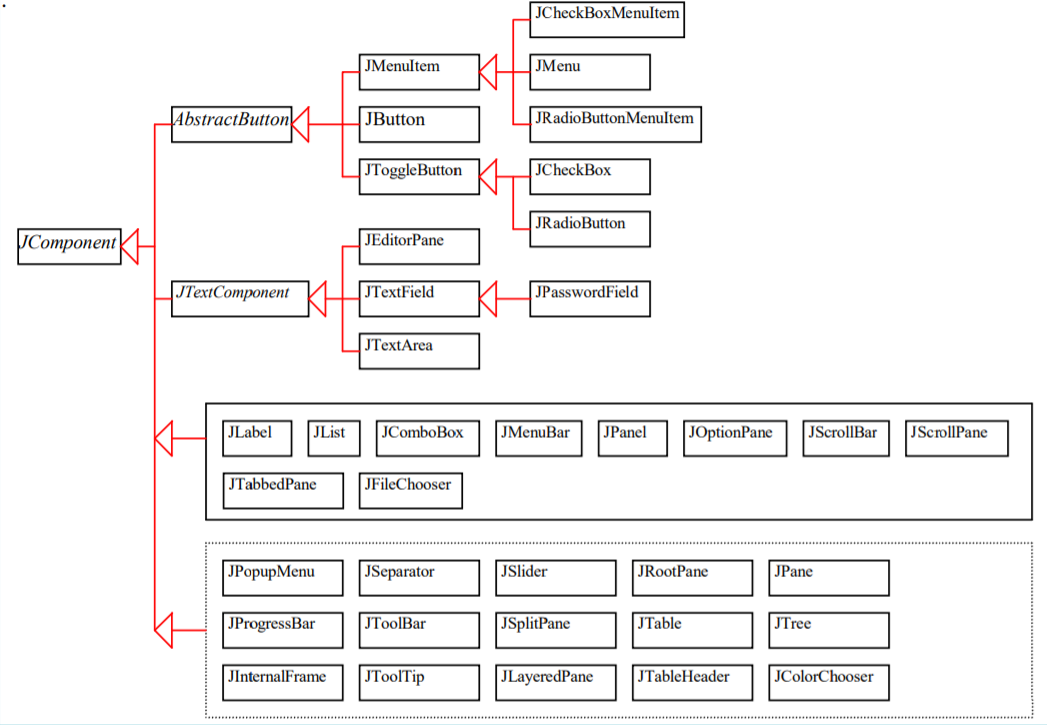
\includegraphics[width=9.3cm]{images/hier}
	\end{frame}
	\begin{frame}{Hierarchy of AWT}
		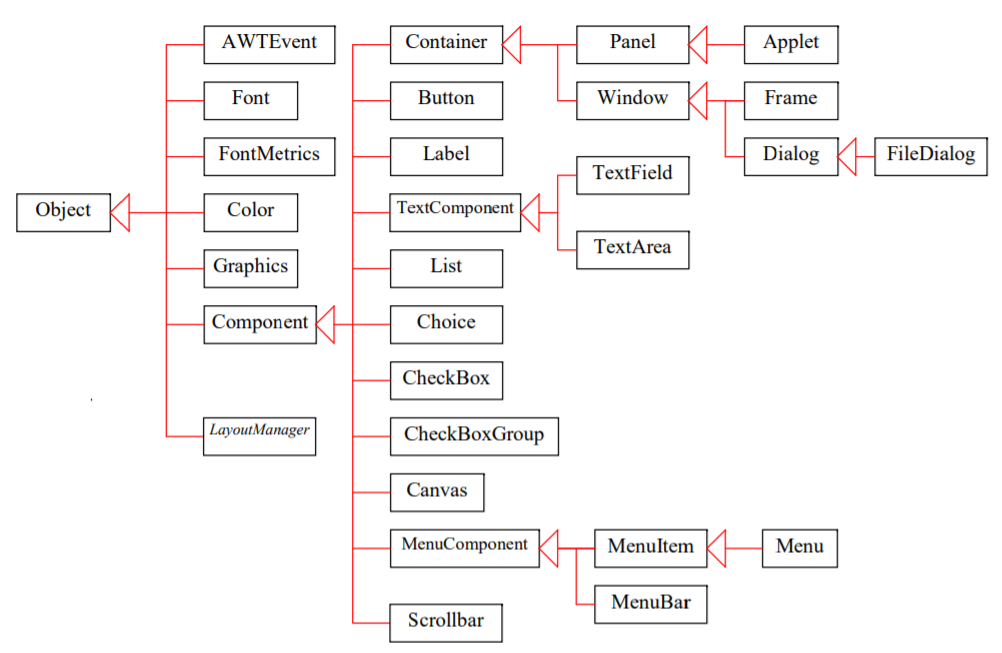
\includegraphics[width=10cm]{images/hierawt}
	\end{frame}
	\begin{frame}{Hierarchy of GUI}
		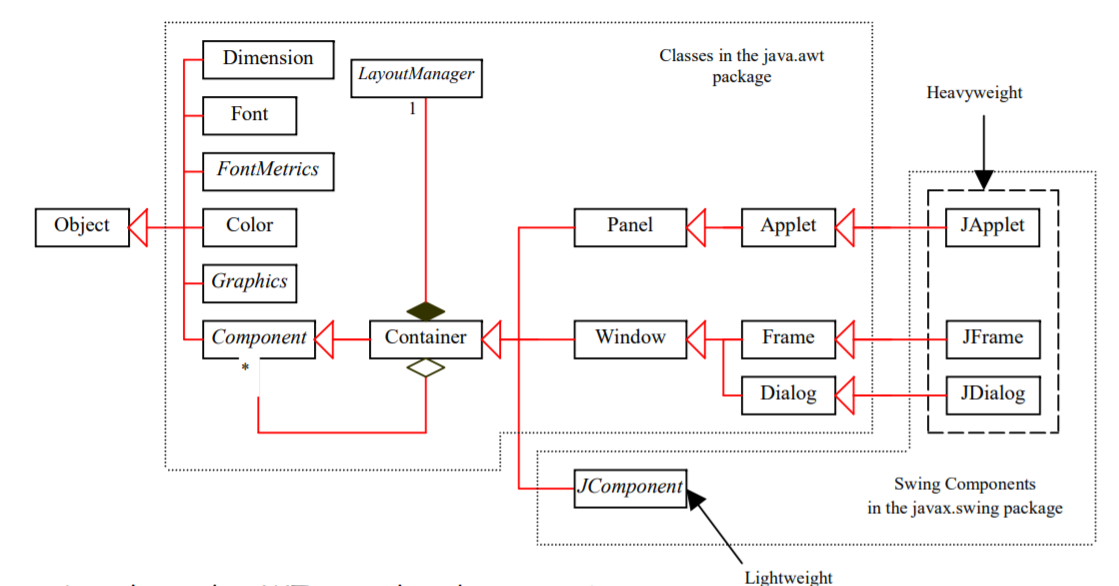
\includegraphics[width=10.7cm]{images/heig}
	\end{frame}
	\begin{frame}{Hierarchy of JFrame}
		\begin{center}
			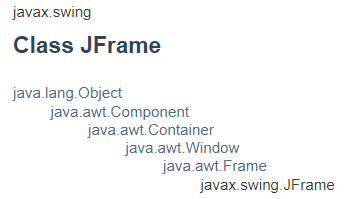
\includegraphics[width=8cm]{images/jerar}
		\end{center}
	\end{frame}
	\begin{frame}{Example of JFrame}
		\begin{center}
			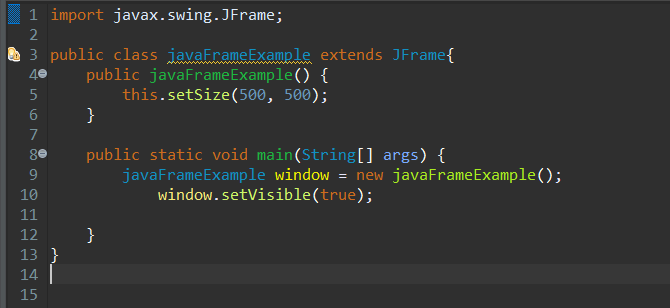
\includegraphics[width=10cm]{images/example1}
		\end{center}
	\end{frame}
	\begin{frame}{Hierarchy of JPanel}
		\begin{center}
			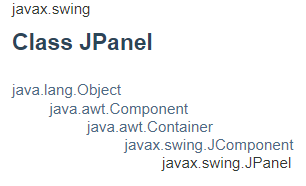
\includegraphics[width=8cm]{images/hierarpan}
		\end{center}
	\end{frame}
	\begin{frame}{Example of JPanel}
		\begin{center}
			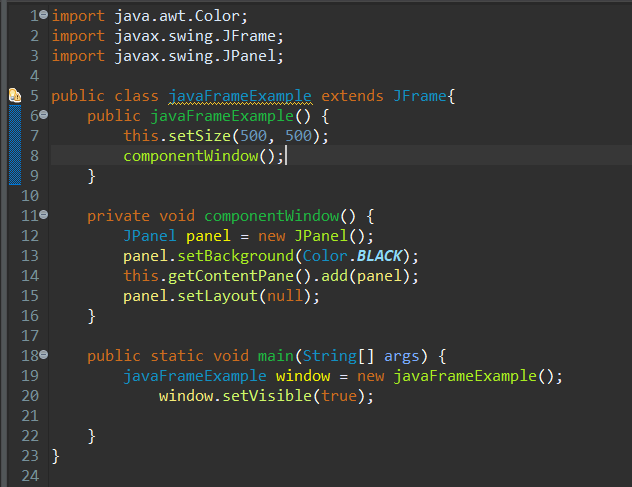
\includegraphics[width=8.4cm]{images/example2}
		\end{center}
	\end{frame}
	\begin{frame}{Hierarchy of Label}
		\begin{center}
			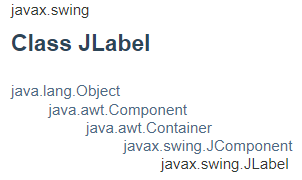
\includegraphics[width=8cm]{images/hierlab}
		\end{center}
	\end{frame}
	\begin{frame}{Example of Label}
		\begin{center}
			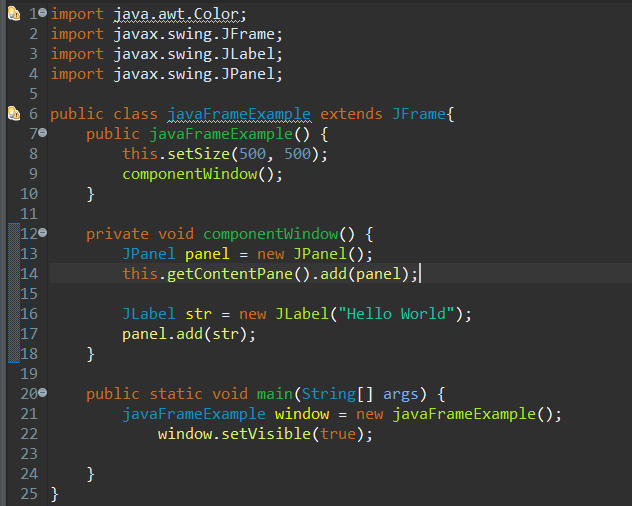
\includegraphics[width=8cm]{images/example3}
		\end{center}
	\end{frame}
	
	\section{References}
	\begin{frame}{References - Web Sites}
		\begin{itemize}
			\item \url{https://docs.oracle.com/javase/7/docs/api/}
			\item \url{https://www.ingeniovirtual.com/la-interfaz-de-usuario-ui-y-su-importancia/}
			\item \url{https://www.fdi.ucm.es/profesor/jpavon/poo/Tema6resumido.pdf}
			\item \url{https://www.youtube.com/watch?v=7q2VBGIKeYc}
			\item \url{https://www.youtube.com/watch?v=RF7Ko3AgRf8&list=PLWtYZ2ejMVJkjOuTCzIk61j7XKfpIR74K&index=87}
			\item \url{https://es.dreamstime.com/sistema-limpio-y-moderno-de-la-interfaz-gráfica-usuario-image118721079}
		\end{itemize}
	\end{frame}

\end{document}